%---------------------------------------------------------
\section{Description}
IzPack est un projet open-source crée en 2001 par Julien Ponge. C'est un generateur d'installeur et il presente a ce titre de nombreuses fonctionnalitees.
\subsection{Générateur d'installeur}
Une application, une fois realisee, necessite un certains nombre d'operations sur la machine pour etre operationnelle. Ces operations vont de la decompression de l'archive dans un repertoire au lancement de script de configuration en passant par la validation de la license et la creation de raccourcis. Creer un installeur pour une application est souvent laborieux et n'apporte que peu de plus-value au programme. 

L'interet d'Izpack reside dans le fait qu'il propose une solution pour creer cet installeur de maniere simple et universelle. En effet, a partir d'une application cree, Izpack est capable de generer un installateur. Cet installateur pourra etre utilise pour deployer l'application sur n'importe quelle machine. De plus, tout type de programme peut etre package, que ce soit une application C++ ou Java. Izpack se chargeant juste de la logique d'installation, il est totalement independant du contenu qu'il installe.
\subsection{Open-source}
Le projet Izpack est placee sous une license Open-source. A ce titre, le code source est librement selon les termes de la license. De plus, une communautee s'est regroupee autour du projet.
\subsubsection{La communaute Izpack}
Cette communaute open-source fait vivre et evoluer le projet. Les personnes rejoignant les projets sont des personnes aux motivations diverses. Ces personnes peuvent etre des passionnes interesse par le projet ou des salaries utilisant Izpack et apportant leurs contribution. Les formes de contributions sont variees. Elles peuvent prendre la forme d'aide aux utilisateurs, de readaction de documentation, de correction de bugs ou d'ajouts de fonctionnalites.
\subsubsection{License}
Izpack est sous license Apache 2. Cette license permet l'acces au code source et l'utilisation libre du logiciel. Il est tout a fait possible de l'utiliser pour une application commerciale voire meme, de modifier les sources pour correspondre a ses besoins. Une importante communaute s'est regroupee autour de ce projet ce qui a permit son evolution jusqu'a maintenant. Si un developpeur apporte des modifications utiles, il est encourage a en faire profiter la communaute, mais ce n'est pas une obligation.
\subsection{Fonctionnalités}
Izpack est un systeme modulaire, il possède de nombreuses fonctionnalités pour creer un installeur adapté a chacun.
\subsubsection{Multi-plateforme}
L'installeur generee par Izpack est un jar (java archive). Il suffit donc que la machine ait un machine virtuelle pour pouvoir lancer l'installation, indépendamment de la plateforme et du système d'exploitation. Il est neanmoins possibles de faire des traitements specifiques a certaines plateforme ou de convertir l'installeur pour etre specifique a une plateforme. 
\subsubsection{Personnalisation}
Izpack propose un ensemble de panels qui vont constituer l'installateur graphique. Chaque panels remplit une fonction specifique. L'aspect global et celui des panels est personnalisable par l'utilisateur via le descripteur XML.
\subsubsection{Internationalisation}
Izpack supporte la création d'installeur multilangues. Pour la localisation, tout repose sur des fichiers XML. Si une langue n'existe pas, il suffit de traduire les phrases/mots dans un fichier xml a utiliser lors de la creation de l'installeur.
\begin{figure}[H]
	\centering
	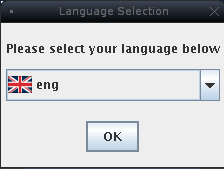
\includegraphics[width=5cm]{../image/LangChoice.png}
	\caption{Exemple de choix de langue avec IzPack}
\end{figure}
\subsubsection{Installation automatique}
A la fin de l'installation, il est possible de générer un script d'installation automatique. Ce script permet de reproduire l'installation réalisée sur d'autres machines.
\begin{figure}[H]
	\centering
	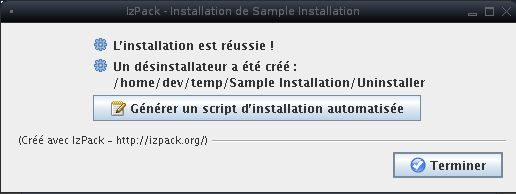
\includegraphics[width=12cm]{../image/SaveInstallXML.png}
	\caption{Fin d'installation, enregistrement du script d'installation automatisee}
\end{figure}
\subsection{Popularité du projet}
Izpack est utilisé dans de grand projets comme Jboss, Xwiki, Glassfish... A l'heure actuelle, les téléchargements mensuels s'élèvent a 25.000.
\begin{figure}[H]
	\centering
	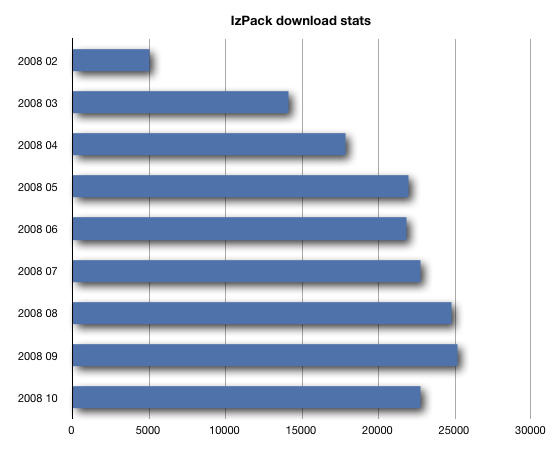
\includegraphics[width=0.6\textwidth]{../image/telechargements.png}
	\caption{Statistiques de telechargements}
\end{figure}
 %---------------------------------------------------------
\section{Architecture}
\subsection{Architecture globale}
Globalement, Izpack possède 2 composants, le compilateur qui va gérer la création de l'installeur et l'installeur.
\subsection{Compilateur}
Le compilateur package l'ensemble des fichiers nécessaires dans un seul fichier jar. Selon la description de l'installation, il va incorporer les panels nécessaires au lancement de celle-ci. Cette partie est utilisee par le developpeur qui souhaite creer un installeur.
\subsection{Installeur}
La partie installation concerne toute la logique et la présentation du processus d'installation. Cette partie sera executer par un utilisateur souhaitant installer le logiciel.
\subsection{Processus d'installation}
Dans un premier temps, le compilateur va compiler l'application.
\begin{figure}[H]
	\centering
	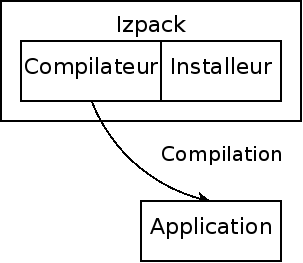
\includegraphics[width=0.4\textwidth]{../image/archi_architecture.png}
	\caption{Phase de compilation}
\end{figure}
L'installateur genere comprend l'application en elle-meme et toute la partie installation necessaire et adaptee au besoin de l'application. Cette application est alors prete a etre deployee sur une autre machine.
\begin{figure}[H]
	\centering
	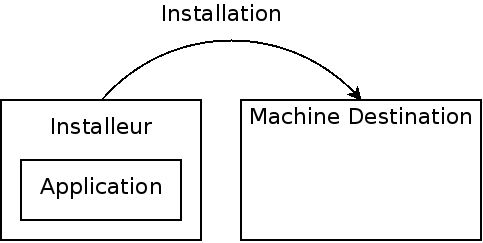
\includegraphics[width=0.4\textwidth]{../image/archi_installation.png}
	\caption{Phase d'installation}
\end{figure}
Le processus d'installation est gere par la partie installeur de Izpack. Cette phase va permettre de deployer l'application sur toute les machines necessaires.
\begin{figure}[H]
	\centering
	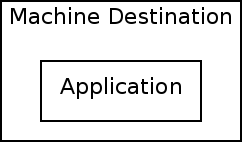
\includegraphics[width=0.3\textwidth]{../image/archi_installe.png}
	\caption{Application deployee}
\end{figure}

\subsubsection{Exemples de panels}
Chaque ecran que verra l'utilisateur est decrit par un panel.
Il existe de nombreux types de panels : des panel pour accueillir l'utilisateur et lui afficher des informations (HelloPanel et HTMLInfoPanel), d'autres pour demander à l'utilisateur des informations (UserInputPanel), etc.
Il existe aussi des panels plus spécialisés. Ainsi, CompilePanel permet de compiler du code java, et ProcessPanel permet de lancer des programmes après l'installation.

% screenshot de panels si on a du temps / de la place

 %---------------------------------------------------------
\section{Exemples d'installation}
De nombreux exemples complets existent, par exemple l'installeur de IzPack, celui de Glassfish, etc. Pour illustrer simplement l'utilisation de IzPack, utilisons plutôt le petit exemple fourni avec le code de l'application.

\subsection{Description du xml}
% un peu porc comme méthode, copier/coller une partie du xml...
% mais je ne vois pas comment présenter ce xml
% et puis ça suffira, au moins pour un premier jet

Ce xml (install.xml) décrit complètement l'installation.
Une balise \verb|info| permet de définir les informations concernant l'application : 
\begin{lstlisting}[language=xml]
<info>
	<appname>Sample Installation</appname>
	<appversion>1.4 beta 666</appversion>
	...
</info>
\end{lstlisting}
Une autre balise, \verb|guipref| permet de définir quelques propriétés de la fenêtre de l'installeur :
\begin{lstlisting}[language=xml]
<guiprefs width="640" height="480" resizable="yes"/>
\end{lstlisting}
Les langues sont définies par la balise \verb|locale| :
\begin{lstlisting}
<locale>
	<langpack iso3="eng"/>
	<langpack iso3="fra"/>
</locale>
\end{lstlisting}
Des fichiers externes nécessaires à l'installation peuvent être définis par la balise \verb|resources| :

\begin{lstlisting}[language=xml]
<resources>
	<res id="LicencePanel.licence" src="Licence.txt"/>
</resources>
\end{lstlisting}
Les panels visibles par l'utilisateur sont décrits dans la balise \verb|panels| :
\begin{lstlisting}[language=xml]
<panels>
	<panel classname="HelloPanel"/>
	...
	<panel classname="FinishPanel"/>
</panels>
\end{lstlisting}
Enfin la balise \verb|packs| contient la description des packs (les differentes parties, optionnelles ou non, de l'application) a installer.
\begin{lstlisting}[language=xml]
<packs>
	<pack name="Base" required="yes">
		<description>The base files</description>
		<file src="Readme.txt" targetdir="$INSTALL_PATH"/>
		...
	</pack>
	<pack name="Docs" required="no">
		...
	</pack>
	...
</packs>
\end{lstlisting}
Bien sûr d'autres options existent, mais celles présentées ici suffisent à créer notre installeur.
\subsection{Génération du jar}
Pour générer notre installeur, il suffit d'avoir de lancer la commande suivante : (l'executable \verb|compile| provient de IzPack)
\begin{verbatim}
$ compile install.xml
.::  IzPack - Version 4.1.0 ::.

< compiler specifications version: 1.0 >

- Copyright (c) 2001-2008 Julien Ponge
- Visit http://izpack.org/ for the latest releases
- Released under the terms of the Apache Software License version 2.0.

-> Processing  : install.xml
-> Output      : install.jar
-> Base path   : .
-> Kind        : standard
-> Compression : default
-> Compr. level: -1
-> IzPack home : .

...

Build time: Tue Mar 10 16:50:27 CET 2009
\end{verbatim}
Cette exécution va produire un fichier install.jar : notre installeur.
\subsection{Installation}
Il suffit désormais de lancer le jar pour installer notre application.
\begin{figure}[H]
	\centering
	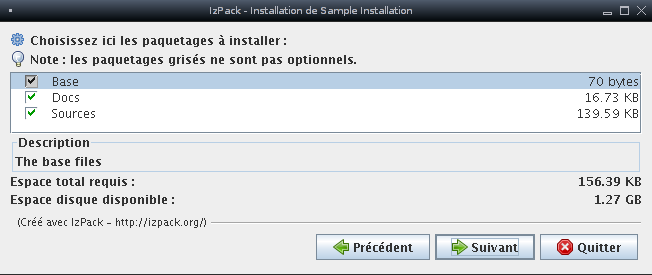
\includegraphics[width=15cm]{../image/installSample.png}
	\caption{Exemple d'installation avec IzPack}
\end{figure}

\subsection{Installation automatique}
En lancant l'installeur avec un script d'installation automatisee en parametre, l'installation est rejouee a l'identique automatiquement.
\begin{verbatim}
$ java -jar install.jar automated.xml
[ Starting automated installation ]
[ Starting to unpack ]
[ Processing package: Base (1/3) ]
[ Processing package: Docs (2/3) ]
[ Processing package: Sources (3/3) ]
[ Unpacking finished ]
[ Writing the uninstaller data ... ]
[ Automated installation done ]
\end{verbatim}


 %---------------------------------------------------------
\section{Problèmes actuels}
IzPack possède, comme tout logiciel, des bugs potentiels ou des améliorations à effectuer.
\subsection{Code obsolete}
Izpack a debute en 2001. A cette epoque, la Jdk en etait a la version 1.3. Il y avait donc des fonctionnalitees absentes a cette epoques comme la genericite. On trouve ainsi du code comportant des tableaux d'objets ou des Vectors.
\subsection{Nanoxml}
Une amélioration possible concerne la gestion des fichiers XML, qui ont une grande importance dans IzPack.

L'abscence de processeur XML integre a la JRE 1.3 a force l'utilisation d'une librairie externe pour traiter les XML. IzPack se base donc sur nanoXML, une librairie Xml, choisie en raison de sa faible taille.
Cette librairie n'est malheureusement plus mise à jour (la dernière mise à jour date de 2003) et possède encore quelques bugs.
De plus, les versions récentes de l'environnement java (JRE) possèdent de base tout ce qu'il faut pour gérer le xml.
Se débarasser de la dépendance à nanoXML et se reposer uniquement sur la JRE permet donc non seulement de rendre la gestion des XML plus sûre et robuste, mais également de diminuer la taille des installeurs générés.
